\documentclass[12pt]{article}
%\usepackage[utf8]{inputenc}
%\documentclass[UTF8]{ctexart}
%\usepackage[UTF8, heading = false, scheme = plain]{ctex}
\usepackage{geometry}
%geometry{a4paper,scale=0.9}
\geometry{a4paper,left=1cm,right=1cm,top=1cm,bottom=2cm}
\usepackage{amsfonts}
\usepackage{color}
\usepackage{url}
%\usepackage{biblatex}
\usepackage{amsmath}
\usepackage{amssymb}
\usepackage{latexsym}
\usepackage[linesnumbered,ruled,lined]{algorithm2e}
\usepackage{cite}
%\addbibresource{ref.bib}
%\bibliography{ref.bib}
\usepackage{caption}
\usepackage{graphicx, subfig}
\usepackage{float}
%\usepackage[fontset=ubuntu]{ctex}
%\usepackage{fontspec}
\usepackage{xeCJK}
%\usepackage[colorlinks,
%anchorcolor=black,
%citecolor=black]{hyperref}
%\setmainfont{SimSun}
\usepackage[section]{placeins}
\usepackage{enumitem}
\usepackage{framed}
\usepackage[framemethod=TikZ]{mdframed}
\usepackage{indentfirst}
\usepackage{setspace}%使用间距宏包
\linespread{1.5}

\title{FM/FFM 概述\cite{FM_Principle_Derivation_Code_Application}}
\author{leolinuxer}
%\date{June 2020}

\begin{document}
%\setlength{\parindent}{0pt}
\maketitle
\tableofcontents

\section{前置知识}
\subsection{线性回归模型}
线性回归模型如下:
$$
y = w_0 + w_1 x_1 + w_2 x_2 + \cdots + w_n x_n \Rightarrow y = w_0 + \sum_{i=1}^nw_ix_i
$$

线性回归模型的假设:
\begin{itemize}
\setlength{\itemsep}{0pt}
\setlength{\parsep}{0pt}
\setlength{\parskip}{0pt}
    \item \textbf{特征之间相互独立不相关};
    \item 特征的作用是可以叠加的;
\end{itemize}

线性回归模型假设特征之间是相互独立的、不相关的。但在某些场景中,特征之间往往是相关的,而不是相互独立的。比如<女性>和<化妆品>,<程序员>与<计算机类书籍>,所以需要特征组合。

特征两两组合,得到二阶多项式如下:
$$
y = w_0 + \sum_{i=1}^nw_ix_i + \sum_{i=1}^n\sum_{j=i+1}^nw_{ij}x_ix_j
$$

其中,$n$ 代表样本的特征数量,$x_i$是第$i$个特征的值,$w_0, w_i, w_{ij}$ 是模型参数。则组合特征的参数一共有$n(n-1)/2$个,任意两个参数是独立的。

\subsection{非负矩阵分解}
非负矩阵:所有元素非负。若 $X$ 是非负矩阵,记作 $X \ge 0$。

非负矩阵分解:给定一个非负矩阵$X \ge 0$,找到两个非负矩阵$W \ge 0$和$H \ge 0$,使得:
$$
X \approx WH
$$

即将非负矩阵$X$分解为两个非负矩阵$W,H$的乘积形式,称为非负矩阵分解。

\begin{framed}
非负矩阵分解的例子如下:

我们把每个 user 表示成一个二维向量,同时把每个 item 表示成一个二维向量,两个向量的点积就是矩阵中 user 对 item 的打分,写成非负矩阵分解形式如下:
\begin{figure}[H]
    \centering
    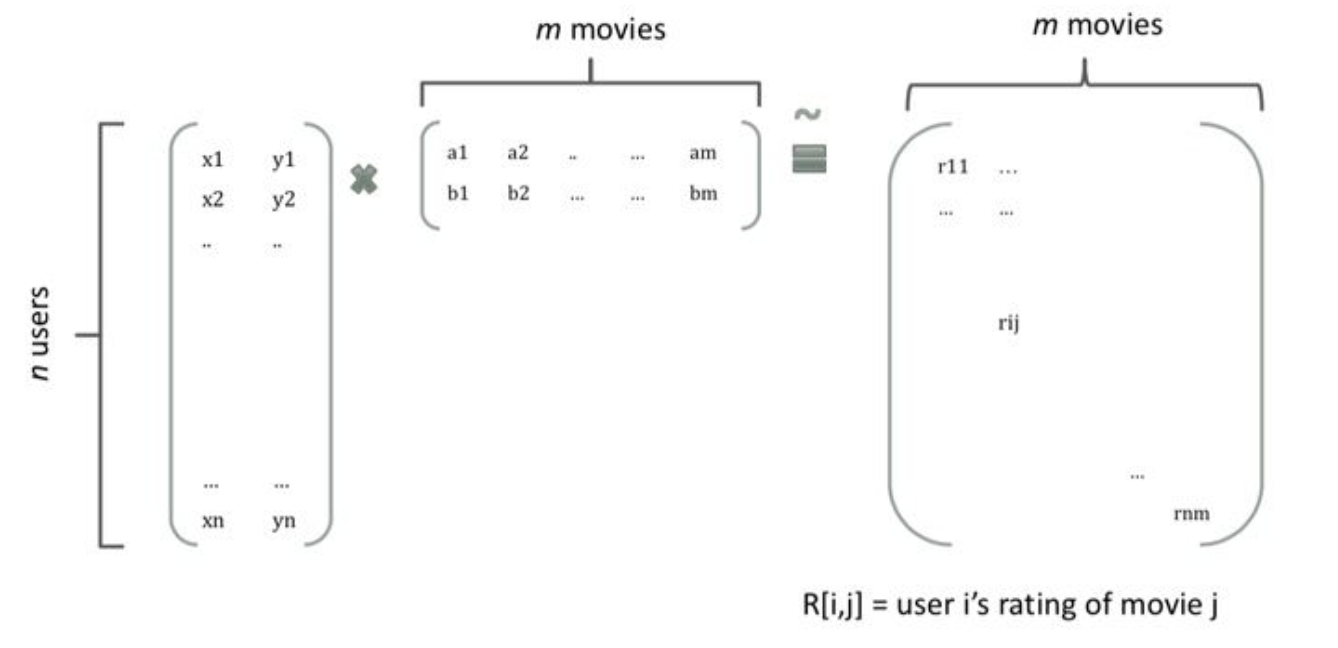
\includegraphics[width=.6\textwidth]{fig/FM_Non_Negative_Matrix_Factorization_Example.png}
\end{figure}
\end{framed}

特征关系的向量化,则得FM模型。

\section{FM模型}
论文:Factorization Machines

因子分解机模型,即Factorization Machine Model,简称FM。

\subsection{FM 模型的方程推导}
上述二阶多项式的二项式参数$w_{ij}$ 可以组成一个\textcolor{red}{对称矩阵} $W$,那么这个矩阵可以分解为:$W = V^TV$,$V$的第$j$列便是第$j$维特征的特征向量,即$W_{ij}$的每个参数都可以表示为:
$$
W_{ij} = < V_i, V_j >
$$
这就是 FM 的核心思想。

即上述二阶多项式可以写成:
$$
y = w_0 + \sum_{i=1}^nw_ix_i + \sum_{i=1}^n\sum_{j=i+1}^n <v_i, v_j > x_ix_j
$$

这边是 FM 的方程。其中,$v_i$ 是第$i$维特征的隐向量,隐向量的长度为 $k$,包含 $k$ 个描述特征的因子;$<\cdot,\cdot>$代表向量点积,即$ < v_i , v_j > = \sum_{f=1}^k v_{i,f}v_{j,f}$。


\subsection{FM 模型的假设}
\begin{itemize}
\setlength{\itemsep}{0pt}
\setlength{\parsep}{0pt}
\setlength{\parskip}{0pt}
    \item \textbf{特征之间两两相关};
    \item 特征的作用是可以叠加的;
\end{itemize}

\subsection{FM 模型的计算}
利用矩阵直观化推导FM模型的计算,具体推导如下。

根据FM 的二阶多项式,扩充后得到如下矩阵:
\begin{figure}[H]
    \centering
    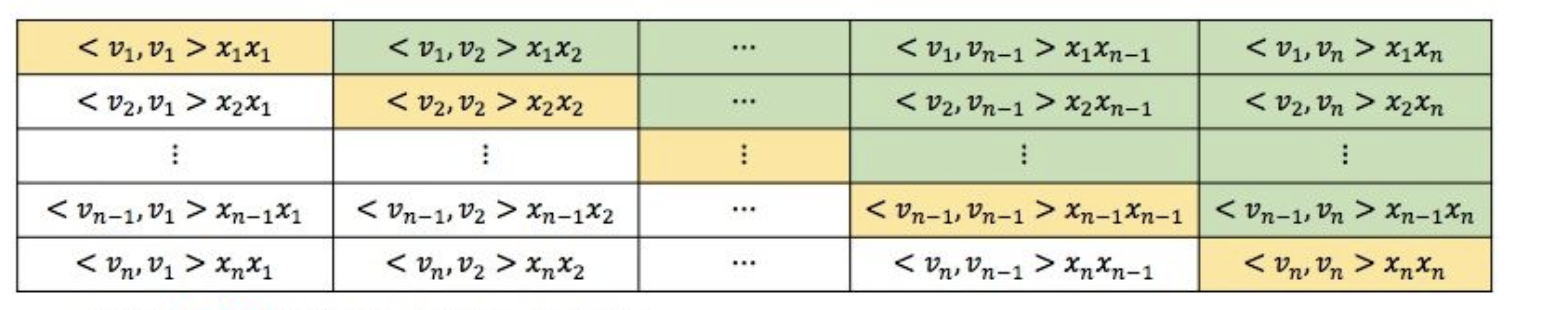
\includegraphics[width=1\textwidth]{fig/FM_Second_Order_Part_Example.png}
\end{figure}

矩阵\textcolor{red}{上三角}(绿色部分)的元素之和即为 FM 的二阶部门:
$$
\sum_{i=1}^n\sum_{j=i+1}^n <v_i, v_j> x_ix_j
$$

等于\textbf{矩阵的全部元素之和减去对角线元素之和,再除以二}:
$$
\sum_{i=1}^n\sum_{j=i+1}^n <v_i, v_j> x_ix_j = \frac{1}{2}\Bigg( \sum_{i=1}^n \sum_{j=1}^n  <v_i, v_j> x_ix_j - \sum_{i=1}^n <v_i, v_i> x_ix_i \Bigg) 
$$

FM模型的二次项化简推导过程如下:
\begin{align*}
\sum_{i=1}^n\sum_{j=i+1}^n <v_i, v_j> x_ix_j &= \frac{1}{2}\Bigg( \sum_{i=1}^n \sum_{j=1}^n  <v_i, v_j> x_ix_j - \sum_{i=1}^n <v_i, v_i> x_ix_i \Bigg)  \\
&= \frac{1}{2}\Bigg( \sum_{i=1}^n \sum_{j=1}^n  \sum_{f=1}^k v_{i,f} v_{j,f} x_i x_j - \sum_{i=1}^n\sum_{f=1}^k v_{i,f} v_{i,f} x_i x_i \Bigg) \\
&= \frac{1}{2}\sum_{f=1}^k \Bigg[ \Big(\sum_{i=1}^n v_{i,f} x_i \Big) \Big(\sum_{j=1}^n v_{j,f} x_j \Big) -  \sum_{i=1}^n v_{i,f}^2 x_i^2 \Bigg] \\
&= \frac{1}{2}
\sum_{f=1}^k \Bigg[ \Big(\sum_{i=1}^n v_{i,f} x_i \Big)^2 -  \sum_{i=1}^n v_{i,f}^2 x_i^2  \Bigg] \qquad(\text{i和j是等价的})
\end{align*}

即 FM 模型方程(时间复杂度为$O(kn^2)$):
$$
y = w_0 + \sum_{i=1}^nw_ix_i + \sum_{i=1}^n\sum_{j=i+1}^n <v_i, v_j > x_ix_j
$$

可以转化为(时间复杂度为$O(kn)$):
$$
y = w_0 + \sum_{i=1}^nw_ix_i +  \frac{1}{2}
\sum_{f=1}^k \Bigg[ \Big(\sum_{i=1}^n v_{i,f} x_i \Big)^2 -  \sum_{i=1}^n v_{i,f}^2 x_i^2  \Bigg] 
$$

同时,在稀疏数据场景下,很多特征为0,所以只需要计算非零特征就行,这样可以极大提升计算效率。

\subsection{FM 模型训练}
FM 可以采用随机梯度下降的方法进行训练。

FM 模型各个参数的梯度如下:
$$
\frac{\partial \hat{y}(x)}{\partial \theta} = \begin{cases}
1 \ \ \qquad\qquad\qquad\qquad\qquad\qquad \text{if} \ \theta \ \text{is} \ w_0\\
x_i \ \qquad\qquad\qquad\qquad\qquad\qquad \text{if} \ \theta \ \text{is} \ w_i\\
x_i \sum_{j=1}^nv_{j,f}x_j - v_{j,f}x_i^2 \ \ \qquad\quad \text{if} \ \theta \ \text{is} \ v_{i,f}
\end{cases}
$$

\subsection{FM模型总结}
\subsubsection{FM模型优点}
\begin{itemize}
\setlength{\itemsep}{0pt}
\setlength{\parsep}{0pt}
\setlength{\parskip}{0pt}
    \item 适用于高度稀疏化的数据场景;
    \item 具有线性复杂度;
\end{itemize}

\subsubsection{线性回归 vs FM}
FM模型由线性回归模型演化出来。二者的最大区别是:线性回归模型的特征独立,而FM模型的特征两两相关。


%\printbibliography
\bibliography{../ref}
\bibliographystyle{IEEEtran}
\end{document}